\documentclass[11.5pt]{article}
\usepackage{charter}
\usepackage{fullpage}
\usepackage[colorlinks=false]{hyperref}
\usepackage{ifthen}
\usepackage{comment}
\usepackage{xeCJK}
\usepackage[title,titletoc]{appendix}

\setCJKmainfont[BoldFont = STSongti-SC-Bold]{STSongti-SC-Regular}
\setCJKfamilyfont{hei}{SIL-Hei-Med-Jian}		%宋体
\setCJKfamilyfont{song}{SimSun}		%宋体
\setCJKfamilyfont{kai}{Kaiti}		%楷体
\setCJKfamilyfont{fang}{song}	%仿宋
\setCJKfamilyfont{li}{song}			%隶书
\setCJKfamilyfont{you}{Yuanti}		%幼圆

\newcommand{\song}{\CJKfamily{song}}	%宋体
\newcommand{\hei}{\CJKfamily{hei}}	%黑体
\newcommand{\kai}{\CJKfamily{kai}}	%楷体
\newcommand{\fs}{\CJKfamily{fang}}	%仿宋
\newcommand{\li}{\CJKfamily{li}}		%隶书
\newcommand{\you}{\CJKfamily{you}}	%幼圆

\setCJKsansfont[BoldFont = STHeitiSC-Medium]{STHeitiSC-Light}

\bibliographystyle{unsrt}
\usepackage{color}
\usepackage{titlesec}
\usepackage{tikz}
\usepackage{tikzscale}
\usepackage{pgfplots}
\usepackage{nomencl}
\usepackage{amsfonts, booktabs,siunitx}
\usepackage{threeparttable}
\usepackage{tabularx}
\makenomenclature

\usepgflibrary{arrows}
\usetikzlibrary{snakes}
\usetikzlibrary{shapes.geometric}
\usetikzlibrary{patterns}
\usetikzlibrary{shapes,arrows,chains}
\usepgfplotslibrary{patchplots,colormaps}
\usetikzlibrary{calc}
\usetikzlibrary{positioning, fit}
\usetikzlibrary{backgrounds}
\usetikzlibrary{intersections}
\usepackage[]{algorithm2e}

\usepackage{flafter}


\newcommand{\todo}[1]{{\color{blue}#1}}
\newcommand{\cmnt}[1]{{\color{red}#1}}

\newcommand{\sectionbreak}{\clearpage}

% math and cite
\newcolumntype{C}[1]{>{\centering}m{#1}}
\usepackage{rotating}
\newtheorem{thm}{Theorem}
\newtheorem{defn}{Definition}
\newcommand{\refsec}[1]{\S\ref{#1}}
\newcommand{\reffig}[1]{Fig.\ref{#1}}
\usepackage{soul}
\usepackage{amsmath}
\usepackage{url}
\usepackage{amsfonts}
\usepackage{amssymb}
\usepackage{amsthm}
\usepackage{soul}
\usepackage{fullpage}
\usepackage[noend]{algorithmic}
%\usepackage{subfigure}
\usepackage[american]{babel}
%\usepackage{csquotes}
%\usepackage{biblatex}
\usepackage{listings}
\usepackage{caption}
\usepackage{subcaption}


\lstset{emph={long, contract, return, uint256, bool, function, if, true,
    else, using, returns, constant, string, public, namespace, struct, for,
    int,char, typedef, void, double, float, static_cast,
    new},emphstyle=\bfseries\ttfamily, 					basicstyle=\ttfamily,
  moredelim=[is][\color{red}]{^}{^}}

%\lstset{language=C++,
                %basicstyle=\ttfamily\footnotesize,
                %keywordstyle=\color{blue}\ttfamily\footnotesize,
                %stringstyle=\color{red}\ttfamily\footnotesize,
                %commentstyle=\color{green}\ttfamily\footnotesize,
                %morecomment=[l][\color{magenta}]{\#}
%}
%\lstset{%
  %escapeinside={(*}{*)},%
%}

\SetKwProg{Contract}{contract}{ \{}{\}}
\SetKwProg{Function}{function}{ \{}{\}}
\SetKwProg{If}{if}{ \{}{\}}
\SetKwProg{Else}{else}{ \{}{\}}
\newcommand{\String}{\KwSty{string}}
\newcommand{\Public}{\KwSty{public}}
\newcommand{\Returns}{\KwSty{returns}}
\newcommand{\Shared}{\KwSty{shared}}
\newcommand{\Constant}{\KwSty{contant}}
\addbibresource{reference.bib}

\begin{document}
\renewcommand{\contentsname}{Contents}
\renewcommand{\abstractname}{Abstract}
\renewcommand{\refname}{References}
\renewcommand{\nomname}{Glossaries}
\renewcommand{\figurename}{Fig.}
\renewcommand{\tablename}{Table}
\renewcommand{\baselinestretch}{1.5}
\renewcommand{\appendixname}{Appendix}

\title{
	Nebulas Technical White Paper \\
	\large A decentralized platform which provides search framework for all blockchains}
\author{Nebulas Team}
\date{September, 2017\\v1.0}

\maketitle
\leavevmode \newline \newline \newline
\abstract{

\todo{
白皮书的摘要,让大家看完摘要后,就对星云链要做的事情一目了然。
}

\todo{TODO是蓝色}


\cmnt{
  注释是红色
}

}


\newpage
\tableofcontents
\newpage
\printnomenclature

\nomenclature{NR}{Nebulas Rank}%
\nomenclature{NF}{Nebulas Force}%
\nomenclature{SCS}{Smart Contract Score}%
\nomenclature{SCR}{Smart Contract Rank}%
\nomenclature{PoW}{Proof of Work}%
\nomenclature{PoS}{Proof of Stake}%
\nomenclature{PoI}{Proof of Importance}%
\nomenclature{PoD}{Proof of Devotion}%
\nomenclature{DIP}{Developer Incentive Protocol}%
\nomenclature{WAA}{Weekly Active Addresses}%
\nomenclature{BFT}{Byzantine Fault Tolerant}%
\nomenclature{NNS}{Nebulas Name Service}%
\nomenclature{NVM}{Nebulas Virtual Machine}

\renewcommand{\nomname}{术语表(按首字母排序)}

\newpage
\section{简介}

\subsection{区块链技术简介}
区块链技术来源于比特币Bitcoin~\cite{Nakamoto2008},其概念由中本聪在2008年提出,是一种去中心化的数字货币。该货币的产生不依赖于任何货币发行机构,而是根据特定算法,依靠大量计算产生,保证比特币网络分布式记账系统的一致性。以太坊Ethereum~\cite{buterin2014ethereum}更进一步,为我们提供了一个可以运行任意类型代码的通用区块链框架。区块链是以比特币和以太坊为代表的数字加密货币体系的核心支撑技术,通过运用数据加密、时间戳、分布式共识和经济激励等手段,在节点无需互相信任的分布式系统中实现去中心化信用的点对点交易、协调与协作,从而解决中心化机构普遍存在的高成本、低效率和数据存储不安全等问题。

需要说明的是,区块链技术本身不是一个全新的技术创新,而是作为一系列技术的组合(包括点对点通讯,密码学,块链数据结构等)产生的模式创新。

\subsection{商业和技术挑战}
以区块链技术为代表的去中心化,自主治理的系统,正在引起越来越多人的重视和研究。当前全球区块链项目已经超过2000个,全球加密数字资产总体价值达到900亿美元。区块链/数字资产领域的用户人群也正在快速增加。从2013年初的全球200万用户,到2017年初的2000万用户。我们认为,在2020年左右,全球区块链/数字资产用户会达到或超过2亿。在2025年前后,全球用户有望达到10亿规模。

随着区块链技术的普及,越来越多区块链技术之上的应用场景被挖掘出来。区块链技术的应用场景已经从最初的数字化货币本身逐步扩展到更多的场景及用户群体中。例如,以以太坊为代表的社区在区块链技术中引入智能合约的概念,Ripple则使用区块链技术实现了全球的结算系统。随着应用场景的多样化,用户对区块链技术的诉求也日益增加,我们已经看到很多挑战。

\paragraph{缺失价值尺度}我们认为,区块链世界需要一个普适的价值尺度,来衡量用户和智能合约的价值,上层应用可以在这个普适的价值尺度上结合自身场景挖掘更深层次的价值,这将带来更多的商业模式的创新,就像Google在互联网世界的兴起一样。

\paragraph{区块链系统的升级}不同于普通软件的版本迭代,区块链系统由于其天生的去中心化特性,无法强制用户升级其客户端及协议。因此,区块链系统中的协议升级往往会引发区块链“硬分叉”或“软分叉”,从而造成巨大的损失,这更进一步限制了区块链系统的应用场景。以比特币为例,社区关于区块扩容至今仍然存在巨大的争议,导致比特币协议进化缓慢,区块容量严重不足,出现过近100万笔交易在交易池等待被写入区块。用户很多时候不得不额外支付高昂的“交易加速费”,严重损害体验性能。另外,从以太坊的“硬分叉”来看,虽然暂时解决了The
DAO问题,但是产生了ETH和ETC“重资产”和社区分裂的“副作用”。

\paragraph{区块链应用生态环境的建立}随着区块链上各种应用(DApp)的快速增长,良好的生态环境是提高用户体验的根本所在。这包括用户如何在海量的区块链应用中检索自己期望的DApp,如何激励开发人员为用户提供更多的DApp,以及如何帮助开发人员更快的构建更好的DApp。以以太坊为例,基于以太坊的DApp总数已经数十万个,试想如果区块链世界中的DApp接近苹果App Store里应用总量规模的话,如何发现并找到用户期望的DApp就是个很大问题。


\subsection{星云链设计原则}
面对上述机遇和挑战,我们要设计一个基于价值激励的自进化区块链系统。具体来说,我们有以下设计原则:
\begin{itemize}
	\item 公正的排名算法,定义价值尺度

我们认为,区块链世界需要一个普适的价值尺度,用于衡量区块链底层简单数据的价值,发现信息的更高维度,从而探索并挖掘区块链世界的更大价值。类似Google的PageRank~\cite{Brin2010}\cite{page1999pagerank},我们也提出区块链世界的NR(Nebulas Rank,星云指数)~(见\refsec{sec:rank})算法,综合考虑了区块链上的资金流动性,以及资金传播的速度、广度和深度,给区块链用户做公正的排名。NR是星云链赋予区块链世界的价值尺度,用来帮助开发者结合自身场景有效衡量区块链中各个用户、智能合约、DApp的重要性。NR有巨大的商业潜力,可以用在搜索、推荐、广告等领域当中。

  \item 区块链系统及应用的自我进化

    我们认为,一个良态的区块链系统及其上的应用应该能够实现自我进化。在较少外部干涉的情况下,实现更快的计算、更强的系统、及更好的体验。我们将这种自我进化的能力称之为NF(Nebulas Force,星云原力)~(见\refsec{sec:nebulasforce})。在星云链的系统架构中,通过在区块结构上的良好设计,基础协议将会成为链上数据的一部分,并通过链上数据的追加实现基础协议的升级;对于星云链中的应用(智能合约),星云链通过在智能合约底层存储支持状态变量可跨合约
    访问的设计,完成智能合约的升级。具备自我升级进化能力的星云链,未来比其它的公有链具有更快的发展速度和更大的生存潜力,同时使得开发者面对漏洞,能够更快的响应 和升级,避免黑客事件给用户带来巨大的损失。

\item 区块链应用生态环境的建设

在星云链中,我们提出了基于账户贡献度的PoD(见\refsec{sec:pod})算法,利用NR的价值尺度评估找出对生态贡献度较高的账户,平等地赋予记账资格,遏制记账权被垄断,并且融合PoS中的经济惩罚,防止公链被恶意破坏,为生态自由发展助力。既能保证较快的共识速度,又能比PoS和PoI更抗作弊,对区块链生态的发展有良好的促进作用。


在星云链中,我们提出面向智能合约和DApp开发者的DIP(Developer Incentive Protocol, 开发者激励协议)~(见\refsec{sec:dip})。DIP的核心思想是对社区贡献度高的智能合约或DApp的开发者,给予他们相应的开发者激励。激励由记账人负责写入区块。

基于Nebulas Rank机制,星云链进一步包含了搜索引擎~(见\refsec{sec:search}),以帮助用户更好的探索区块链中的高价值应用。

\end{itemize}


考虑到以太坊已经有巨大的生态,是一个非常成功的公有区块链平台。星云链希望尽可能的借鉴以太坊等其他区块链系统的优秀设计,从智能合约编程上完全兼容以太坊,使得基于以太坊开发的产品能够零成本的迁移到星云链上。


基于上述设计原则,我们试图构建一个基于价值尺度的区块链操作系统及搜索引擎。本白皮书详细描述了星云链中关于技术的细节,其中\refsec{sec:rank}描述了一种可能的价值尺度及其算法Nebulas
Rank,\refsec{sec:nebulasforce}描述了星云链的自我进化能力Nebulas Force,
\refsec{sec:dip}、\refsec{sec:pod}、\refsec{sec:search}、\refsec{sec:tools}描述了星云链在建设区块链应用生态圈的的设计和构想,最后,\refsec{sec:nascoin}描述了星云链的代币NAS。

\section{Nebulas Rank算法}


\subsection{Introduction} \label{sec:intro}
Ranking nodes in complex network has been a fundamental concern in various applications. One canonical example is PageRank\cite{Brin2010}\cite{page1999pagerank}, which is the core algorithm for Google and other search engines\cite{langville2011google}. Besides, by ranking algorithm, people also want to find out the most influential spreaders in epidemic and information network\cite{doerr2012rumors}\cite{Kitsak2010}, the most acknowledged scientist by the citation network or co-author network\cite{walker2007ranking}\cite{chen2007finding}\cite{Radicchi2009}, the most important cities in the transportation network\cite{guimera2005worldwide}, the most important vertices in metabolic network\cite{ivan2010web}, the top VC firms by co-investment\cite{Bhat2012} etc. And when it comes to designing \textbf{Nebulas Rank} algorithm for blockchain world, decades of researches have enlightened us with many measurements like degree centrality\cite{freeman1979set}, eigenvector centrality\cite{bonacich1972factoring}, Katz centrality\cite{katz1953new}, PageRank\cite{Brin2010}, HITS\cite{kleinberg1999authoritative}, closeness centrality\cite{sabidussi1966centrality}, betweenness centrality\cite{freeman1977set}\cite{freeman1978centrality}\cite{freeman1991centrality}\cite{noh2004random}\cite{newman2005measure}, etc. Before building our algorithm on the top of them, however, we still need to answer two questions:

\begin{enumerate}
\item What properties are embedded in the network?
\item What value should the rank represent?
\end{enumerate}

For the first question, \textbf{Nebulas Rank} uses the transaction graph of blockchain system, which is generated by the transaction history during the past period. We compare blockchain transaction graph with others in three aspects. First, as node representing blockchain system accounts and edges representing money transferring between two accounts, basically, the graph is a weighted directed graph, bearing large difference from social network\cite{Ugander2011} and similarity with webpage network\cite{} in terms of topology. An asymmetric, i.e. directed, edge represents the imbalanced ability of giving or collecting money between two nodes. And the edge weight is of absolute amount, rather than probabilistic, which also enables disparity of link quality among edges. Directly applying standard algorithms could discard these important information. Second, since the graph reveals trajectory of money flow, it could be presumed that Exchanges are highly ranked, whereas such accounts are willing to swap money with any client. Thus anyone can acquire unlimited links from those existing important nodes without much cost. Along with the anonymity of typical blockchain systems, sybil attackers could make large amount of transferring with a big Exchange account, in order to improve his influence such as PageRank. (It is still hard to receive money from a large number of non-sybil nodes, though.) This is an essentially difference from previous researches' assumptions\cite{}. For example, \cite{} assumes that in an online social network with subscription\cite{}, it costs no effort to follow an opinion leader, while attracting a verified opinion leader's attention is not an trivial thing. Third, being different from Bitcoin\cite{}, the newly invented blockchain systems such as Ethereum\cite{} introduces "contract" as a new type of account. After a normal account invoking some method of a contract, a sequence of consequent callings will be raised forming part of a call graph. Unlike Bitcoin\cite{} transaction graph, which only contains money transferring, Ethereum call graph/network also represents dynamic programming calling. We believe such network embeds more information and should be useful to measure a DApp or smart contract's value.

For the second question, \textbf{Nebulas Rank} aims to measure the value of users, and smart contracts \cite{} in blockchains. For normal accounts, we define value by two aspects: \textbf{Liquidity}, which stresses the ability to control digital assets flow of high quality; \textbf{Propagation}, which focus more on the spreading influence. For smart contracts, we also consider \textbf{Interoperability} as a measurement. There are three-fold purposes in \textbf{Nebulas Rank}: 1) to be a good metric for blockchain accounts and smart contract search engine; 2) to provide a trustful criteria in PoS\cite{poelstra2015stake} consensus protocol, where only high ranked nodes should be eligible to become a validator; 3) DIP[TBA]. In this version of white paper, we does not include smart contracts and DIP, as they are of another independent interest and would be presented later. So next all we will discuss is about normal accounts ranking only.

As revealed in \cite{Borgatti2005}, most centrality measures can be classified by their type of network flow. From the dimension of diffusion mechanism, traffic flow can spread by different kinds of duplication or transfer. Another spectrum is the trajectory of flow, which can be either paths, trails or walks. Essentially, blockchain transaction graph is the trajectory of money exchange, which falls into the classification of "transfer walk". Imagine an amount of money enters the network. Then the owner node divides the money and transfers it to its neighbors or keep it with different probabilities, More specifically, the money is divisible, imperishable and non-replicable and each step of walk is random due to the limit of local information. So with the context of "transfer walk", we roughly represent the Liquidity by the amount of flows a node "controls" and the Propagation by the amount of flux over a node. Additionally, however, although the graph represents money exchange, it may as well be seen as other flow types which might outputs better ranking. For example, information flows with "parallel replication along paths", since one may also argue that accounts transfer money because of knowing each other and exchanging information.

Following are our solutions to the challenges described above.

First, in order to turn a list of transaction records into a graph, we keep the transferring value as the edge weight and embed temporal information into node's property. We assign each directed edge's weight as the sum of largest $K$ transactions amounts from source account to target account during the past $T$ days. Then we reduce each edges' weight by its target's "coinage" (see \refsec{subsec:coinage}) and outgoing amount(see \refsec{subsec:limit}) as well as an encouragement function (see \refsec{subsec:encouragement}). By this mean, a directed weighted graph can be generated and some undesired activities can be mitigated:
\begin{itemize}
	\item By setting a time window of $T$ days and treating transactions, old and new, impartially, a node is encouraged to keep active all the time;
	\item Because at most $K$ transactions between each two nodes are counted, simply transferring over edges repeatedly does not improve links' quality;
	\item In order to get higher coinage, money needs to stay in place for a while, which slows down sybil attacks such as transferring money along loops or interact frequently with Exchange service node
	\item Accounts are encouraged to transfer out enough amount of money in order not to get their in-links reduced, which contributes to better money circulation.
\end{itemize}
We will talk about details of transaction processing method in \refsec{sec:txg}.

Second, with graph generated, we measure each node's importance based on Weighted LeaderRank algorithm\cite{Chen2013}\cite{Li2014}. LeaderRank is a simple variant of PageRank, which adds a ground node into the network and connect the ground node with each non-ground node. It substitutes PageRank's damping factor by links throughout ground node, which is said to be more effective in computing, robust against manipulations and noise than PageRank algorithm\cite{Chen2013}. The intuition for both LeaderRank and PageRank is random walk and Markov Chain. By PageRank, from each node, the probability of jumping to an arbitrary node is the same (or equal to 1 if there is no out links \cite{Kim2002}). Whereas by LeaderRank\cite{Li2014}\cite{Chen2013}, different nodes adopt different arbitrary transition probabilities. For example, we could allow a node with more in-links to receive more from the arbitrary transition. This is more plausible in the context of blockchain, since an account with little money transferred in is less trustable. Also, imagine a node receiving much money but hardly spend it. We suppose such account has more "surplus value" and assign it with more arbitrary outgoing probability. We will talk about the details of LeaderRank scheme in \refsec{sec:leaderrank}.

LeaderRank is a measurement of the node flux. Intuitively, money flows in and out from one node in a continuous and dynamic pattern, and LeaderRank observes the steady amount of money passing by a specific node. From another perspective, mode flux means more control. The LeaderRanks algorithm matches both our goals of measuring \textbf{Liquidity} and \textbf{Propagation}. Although some other betweenness based algorithm such as flow betweenness\cite{} and random walk betweenness (aka. current flow betweenness)\cite{} may be more suitable to represent the flow controlling ability i.e. \textbf{Liquidity}, such measurements are quite computational intensive. So we don't adopt them for now. Besides, there are some more thinkings during the design of \textbf{Nebulas Rank}. For example, the network clustering may also be helpful to lower rank spam nodes\cite{}. But it is also defective to overexploit the clustering effect. All issues will be discussed at \refsec{sec:discuss}.

\st{Our experiment results shows that ...... }

The rest of paper is organized as follows. \refsec{sec:related} introduces the related works. Then in \refsec{sec:txg}, we define the network topology and weight based on blockchain transactions. And in \refsec{sec:leaderrank}, LeaderRank with schemes designed for \textbf{Nebulas Rank} is introduced. In \refsec{sec:exp}, we show our experiment results. And Finally we give all discussions and conclusions in \refsec{sec:discuss}

\subsection{Related Works \label{sec:related}}
Centrality, the core ranking index, is a most studied concept in network science since decades ago\cite{newman2010networks}. There are a body of literatures introducing various centralities, including degree centrality\cite{freeman1979set}, eigenvector centrality\cite{bonacich1972factoring}, Katz centrality\cite{katz1953new}, closeness centrality\cite{sabidussi1966centrality}, betweenness centrality\cite{freeman1977set}\cite{freeman1978centrality}\cite{freeman1991centrality}\cite{noh2004random}\cite{newman2005measure}, PageRank\cite{Brin2010}, HITS\cite{kleinberg1999authoritative}, SALSA\cite{Science2001}, etc. It is fundamental to clearly classify these measurements by a unified framework. \textcite{Borgatti2005} adopts a network flow based view to classify the centrality measurements by two categorical dimensions: material flowing by parallel duplication, serial duplication and transfer; and trajectory following geodesics optimum, path, trail and walk. \textcite{Borgatti2006} propose a unified framework with four dimensions from the perspective of graph theory. \textcite{Lu2016} review representative centrality algorithms and classified them into those only based on structural information, those driven by Markov dynamics, those by looking at the effect of removing nodes, those with dynamics-sensitivity and those trying to identify more than one node. With a hierarchical understanding of centrality algorithms, we are able to choose appropriate strategy according to the network scenarios. \textbf{Nebulas Rank}'s scenario is the money exchange flow network mentioned in \cite{Borgatti2005}.

Since Bitcoin\cite{Nakamoto2008} system released in 2009, researchers have done some statistical and empirical analysis on Bitcoin's transaction graph\cite{Ron}\cite{Haslhofer}\cite{NielKondor2014}\cite{Baumann2014}, and some use the transaction graph structure to discuss anonymity in Bitcoin\cite{Meiklejohn2013}\cite{Ober2013}\cite{pham2016anomaly}\cite{Fleder2015}\cite{Ferrin2015}. After other cryptocurrencies emerged and become popular, transaction graph analysis is conducted with more blockchains\cite{Chang2017}\cite{Anderson2016}. \textbf{Nebulas Rank} adopts their transaction graph concept, i.e. Entity Graph in \cite{Tschorsch2015}, with minor revisions. That is, each account, or set of accounts belonging to the same people, is mapped as a node. And each directed edge represents the intensity of transferring between two accounts. Actually before blockchain system like Bitcoin was invented, scientists have tried to study some financial networks among banks and global trading entities\cite{propper2008towards}\cite{Boss2004}\cite{Serrano2007}\cite{Bech2008}\cite{Fagiolo2009}\cite{Morten2006}\cite{Boss2004a}\cite{Krempel2002}\cite{Serrano2003}. Comparing with blockchain transaction networks, these early studied finical networks are defined not only by transferring activities, but also by lending-based relationship. Moreover, the scale of these networks is much smaller. To conclude, there is rarely research work proposing custom ranking method for large scale transaction graph, especially blockchain transaction graph.

The most relevant work with \textbf{Nebulas Rank} is NEM\cite{nem}'s Proof-of-Importance scheme. It adopts NCDawareRank\cite{Nikolakopoulos2013}, which exploits the clustering effect of network topology, as the ranking algorithm, with clustering algorithm based on SCAN algorithm\cite{xu2007scan}\cite{shiokawa2015scan}\cite{chang2017mathsf}. And \textcite{Fleder2015} uses PageRank\cite{Brin2010}\cite{page1999pagerank} as an assisting metric to discover interesting addresses and analyze their activities. However, both NCDawareRank and PageRank are ranking algorithms for webpage network. As we already mentioned in \refsec{sec:intro}, blockchain transaction graph is very different from webpage network. And although community structure does exist in transaction graph and should be helpful to handle with spam nodes, it does not suit the consensus purpose mentioned in \refsec{sec:intro}. Because in order to compute "unforgeable" node importance, accounts controlled by a single "real world" entity should be guaranteed to be mapped to the same cluster. However it is key difficulty to connect blockchain world with the "real world", and thus there is no proper objective definition for clustering problem. Therefore current clustering algorithms cannot provide meaningful and trustful result. Moreover, \cite{Fleder2015}'s work does not provide an automated framework to identify important nodes. Instead, it still needs manual analyzing with the help of PageRank, which does not match \textbf{Nebulas Rank}'s context.

The algorithm we choose is LeaderRank\cite{Chen2013}\cite{Li2014}. It is a simple variant of PageRank\cite{Brin2010}\cite{page1999pagerank}. In PageRank, initially every node gets one unit rank value. Then at each iteration, every node distributes its rank value equally to its directed neighbors. To deal with dangling node problem, there is a damping factor, where every node distribute a specific proportion of its rank value to all nodes equally in the network. \textcite{Chen2013} propose a simple yet effective modification on PageRank's damping factor and call it LeaderRank. Then \textcite{Li2014} extend LeaderRank to weighted case and further improve its performance. By weighted LeaderRank\cite{Li2014}, an additional ground node is added and a bidirectional link is added between every node and ground node. Every edge targeting to ground node is of same weight and every edge from ground node is weighed positively proportional to target node's in-degree. LeaderRank is more resistant against manipulation and noisy data than PageRank\cite{Chen2013}\cite{Li2014}\cite{Lu2016}. In terms of computation, LeaderRank can be seen as PageRank with one more node and set damping factor to be zero. And thus it is easy to implement and very scalable. We will modify LeaderRank a little and discuss more on its weighting scheme at \refsec{sec:leaderrank}.

\subsection{Transaction Graph} \label{sec:txg}

\subsubsection{Transactions}\label{subsec:transfer}
The input data for \textbf{Nebulas Rank} are all the transaction records, i.e. token transferring, during the past $T$ days, denoted by a set of tuples:
$$
	T_{xs}^{all} = \{(s,t,\tau, a), \tau = Today-T \dots Today \}
$$
, where $s$, $t$ and $a$ are the source account, target account and amount of an transfer, respectively.

Further, we filter transactions, providing that self transfer and zero amount transfer are excluded:
\begin{align}
	T_{xs} = \{(s,t,\tau, a)| s \neq t \land a > \Phi \land (s,t,\tau, a) \in T_{xs}^{all} \}, \Phi = 0
\end{align}

\subsubsection{Transactions Aggregation} \label{subsec:aggreate}
 Based on transactions defined above, we construct the directed weighted transaction graph $G=(V, E, W)$, where node set, edge set and weight on edges are denoted by $V$, $E$ and $W$ respectively. We also denote that $N = |V|$ and $M = |E|$.

Each vertex $v \in V$ represents one individual account's address. Each edge represents the transferring intensity between two accounts. Consider $e=(s,t) \in E$, this edge is directed, and naturally, the weight of it should be determined by all related transactions, i.e. $(s,t,\tau, a) \in T_{xs}$. To compute edge $(s,t)$'s weight, we take the sum of top $K$ amounts out of all related transactions:
\begin{align}
w_e = \sum_{i=1}^K a_i, s.t. a_i \in \{a|(s,t,\tau,a) \in T_{xs} \} \land a_1 \geq a_2 \dots
\end{align}

By this mean, the link between two nodes is bi-directed and asymmetric, with top $K$ transactions along each direction aggregated to become the weight. This is different from NEM, which all transfers amounts between two nodes are aggregated into one unilateral edge's weight\cite{nem}. We presume NEM's solution is vulnerable to manipulations, since only a simple triangle loop will enhance edges' weight into infinity. We will show the advantage of our aggregation method in \refsec{} \st{experiment confirming why doing so}

\subsubsection{Temporality Embedding} \label{subsec:coinage}
We noticed that the transactions happens with timestamps. So we try to embed this temporal information as a property of nodes. For each account, we calculate its coinage by the following pseudo-code.

\st{formula} \st{Defined as $C_v$ normalized by max}

\begin{figure}
\includegraphics{coinage.pdf}
\end{figure}


The intuition of coinage is \st{insights}.

Besides, we conjecture that reducing each transaction's contribution according to its block height, like NEM does\cite{nem}, encourages users to postpone their transferring until the last day of period, which will cause unnecessary confusion. Instead, \textbf{Nebulas Rank} treats each transaction equally, which encourages every account to keep active all the time.

We will talk about the coinage exploitation in \refsec{subsec:reduction}. And we will show the advantage of our solution in \refsec{} \st{experiments confirming the effect of coinage}.


\subsubsection{Encouragement Function}\label{subsec:encouragement}
\st{formula and intuition} \st{defined as $B_v$ normalized by max}

We will talk about how we apply the encouragement function in \refsec{subsec:reduction}. And we will show its advantage in \refsec{} \st{experiments confirming the effect of encouragement function}.

\subsubsection{Exploiting Nodes' Property} \label{subsec:reduction}
We defined two node properties $C_v$ and $B_v$ in \refsec{subsec:coinage} and \refsec{subsec:encouragement}, respectively. Then we reduce each edge's weight by its target node's properties:
\begin{align}
	w_{(.,v)} \leftarrow w_{(.,v)} \times ln(1 + \frac{C_v + B_v}{2})
\end{align}

\subsubsection{Mitigating Dormant Effect} \label{subsec:limit}
Consider a node receiving a large amount of money but does not spend any. This node forces its money to be "dormant " and prevents money from being circulated, which contradicts with \textbf{Nebulas Rank}'s purpose(\refsec{sec:intro}). Thus we need to mitigate this dormant effect. In detail, we consider 1-hop local information of each node, limiting the amount of its in-transfers by the total amount of its out-transfers:

\begin{align}
\label{formula:limit}
w_{(.,v)} \leftarrow  \frac{w_{(.,v)}}{\sum_u(w_{(u,v))}} min\{ \sum_u{w_{(v,u)}}, \sum_u{w_{(u,v)}} \}.
\end{align}

Intuitively, such restricting method is reasonable: 1) Imagine two phases for a piece of blockchain token. First it is made out of thin air, which is as the reward of the system. Second it is either circulated around the whole network, which almost never stops being transferred from accounts to accounts, or enters dormant state, which the last owner does not spend it out. Formula \ref{formula:limit} does not affect the first phase, as edges weights can only be reduced as in-links. And in the second phase, accounts are encouraged to spend enough money in order to improve their in-link quality. 2) From the perspective of money flow, only circulated money should be counted. Nodes with dormant money does not control much of the network flow. That is, deleting these nodes does not affect interactions among other nodes. So formula \ref{formula:limit} conforms with \textbf{Nebulas Rank}'s Liquidity value (\refsec{sec:intro}).

We will show the how \textbf{Nebulas Rank} benefits from mitigating dormant effect in \refsec{}.

\st{will this affect wgc????}

\subsection{LeaderRank} \label{sec:leaderrank}
We build our scoring algorithm based on LeaderRank\cite{Li2014}\cite{Chen2013}. It does minor modification on the famous PageRank algorithm\cite{Brin2010}\cite{page1999pagerank}. The ranking algorithm can be understood as a Markov chain. States are nodes. Transition probability is proportional to the weight of some node's out-edge. By PageRank, if there is no out-edge from some node, aka Dangling Node\cite{Kim2002}, the strategy from transition probability from corresponding node is that evenly among all other pages


 It can be described  by an iterative process:

\begin{align}
	R_j^{t+1} = \sum_u R_j^t \times \frac{ w_{(j,i)} }{ \sum_k w_{(j,k)} }
\end{align}


\st{explain}

We add one ground node $\mathcal{G}$ into the network, and double link it with every other node. First every non-ground node gives and receives an amount of "altruist" money to the the ground node: $\forall v \in V$, $w_{(\mathcal{G}, v)} = \beta \times mean(W)$, $w_{(v,\mathcal{G})} = \alpha \times mean(W)  $. Then every non-ground receives an amount of "bonus" money from the ground node:  $\forall v \in V$, $w_{(\mathcal{G}, v)} \leftarrow w_{(\mathcal{G}, v)} + \gamma \sum_u w_{(u,v)}$. Then \st{mathmatical proof to adopt power method}.

Thus we build a probability matrix based on the graph with ground node. $H_{(N+1) \times (N+1)} = h_{ij}$, $\forall i,j \in V \cup \{\mathcal{G}\}$, $h_{ij} = w_{ji} / \sum_k{w_{jk}}$. It holds that $\forall v \in V \cup \{\mathcal{G}\}$, $\sum_u{h_{uv}} = 1$.

Using power method as follows, we are able to compute the rank for every node:

Initially we have $P^0 = \mathcal{R}^{n \times 1} $, $\forall v \in V, P_v^0 = 1/n, P_{\mathcal{G}}^0 = 0$;
At each iteration $i=1,2 \dots $, $P^i = H \times P^{i-1}$;
After convergence, we get $P^*$, then distribute ground node's rank among every other node evenly, i.e. $\forall v \in V$, $P^*_v \leftarrow P^*_v + \frac{P^*_{\mathcal{G}}}{N}$.


\st{explain}

 the out link weight from each node to ground node is of the same amount, causing different damping factors for each node, i.e. the less a node's out degree is, the more likely it jumps to an arbitrary node. Considering receiving from this kind of arbitrary jumping, PageRank actually gives high probability to nodes with lower in-degree, which may be overestimate the quality of new nodes.[formula support here] But Weighted LeaderRank\cite{Li2014} assigns more probability to nodes with more in-degree. In the context of blockchain transaction, new accounts are more likely to be sybil nodes, thus the latter is more plausible. However, there could also be more weighting scheme for LeaderRank. \st{Consider a node with large incoming value but little outing value. Such node is preventing money from flowing, so it is explainable to distribute its "surplus value", namely incoming value minus outing value, to the ground node.} In our design, each node sends and receives "basic flow" of same amount to and from the ground node. And each each node also receives "bonus flow", which depends on the node's in-degree, from the ground node. The rank in steady state represents the expected amount of money flow through every node. We will talk about the detail of our Weighted LeaderRank in



\subsection{Experiments} \label{sec:exp}
\subsubsection{Ethereum Stats}
\st{degree - avg neighbor degree and dynamics; hhi}
\subsubsection{Exploitability of 1-hop Local Information}
\subsubsection{Noise Resistance}
\subsubsection{Sybil Attack Resistance}
\st{all with comparison}

\subsection{Discussions And Conclusions} \label{sec:discuss}

\newpage
\section{PoD贡献度证明共识算法}
\label{sec:pod}

\subsection{设计目标}
\label{pod:goals}

共识算法作为区块链的基石之一,快速和不可逆是我们重点关注的目标。除此之外,为了更好地建设公链生态,我们认为公平性同样重要,如果大资本可以轻松占据公链中区块共识的话语权,那么会有很多公链上的开发者和用户的利益无端受损,一个不能保障公链建设者利益的生态,很难沉淀出价值深度,和星云链设计原则相违背。所以我们在设计共识算法时,在优先保证快速和不可逆的情况下,将尽可能追求公平性,维护公链建设者的利益。

\subsection{常用共识算法的缺陷}
\label{pod:weakness}

我们试图在较为常用的共识算法中找到符合我们设计目标的选择,但是这些算法和我们的目标多少都有些差距。

PoW (Proof of Work)工作量证明共识算法为零和博弈,采用竞争性哈希计算来确定记账人,导致了整个生态每次出块时都有大量电能在竞争中被无端消耗,挖矿成本高,而且速度受限。如果把公链参与者作为整体来看,随着参与挖矿的节点增加,每个节点获得记账权的概率将会减小,那么PoW协议下生态维持平稳出块的成本将会持续升高。不断增加挖矿难度的Bitcoin早晚需要面临矿机收益入不敷出的情形,而Ethereum则早已在考虑使用新的PoS共识算法Casper~\cite{casper}来逐步取代现阶段的PoW共识~\cite{buterin2013ethereum}。可见,从挖矿速度和经济成本角度,PoW都不利于公链生态的长期快速发展,和我们“快速”的目标不相符。

PoS (Proof of Stake)股权证明共识算法试图采用资产的多寡来取代算力的作用,按照币龄或者押金数额来分配获得记账权的概率,现阶段Peercoin~\cite{king2012peercoin}和Ethereum的Casper协议都采用了PoS共识算法。这种算法解决了PoW高能耗的弊端,但很直观地放大了资本对记账权概率分配的影响,相较于PoW,在PoS下大资本更容易占据生态的话语权,形成大集团垄断,可能会对生态的建设者的利益造成损害,不利于公链生态的价值沉淀,同样和我们“公平性”的目标不相符。

PoI (Proof of Importance)重要度证明共识算法最早由Nem提出~\cite{nem},不同于PoS,PoI中引入了账户重要程度的概念,使用账户重要性评分来分配记账权的概率。这种算法解决了PoW的高能耗弊端,减缓了PoS的资本垄断危机,但暴露了nothing-at-stake的问题,作弊者逆转一个区块的成本被大大降低,和我们“不可逆”的目标不相符。

综上,鉴于常用共识算法和我们目标存在差距,我们提出了基于账户贡献度的PoD (Proof of Devotion)算法,将评估账户综合影响力的PoI和具有严格经济惩罚的PoS相融合,利用PoS强化PoI的不可逆性,使用PoI反向遏制了PoS的垄断性,以此为生态自由快速发展助力。

\subsection{PoD算法设计}
\label{pod:design}

\subsubsection{新区块产生}
\label{pod:design:block}

类似PoI共识算法选取重要性高的账户,PoD将选取生态中贡献度较高的账户,不同之处在于,PoD赋予选取出来的账户平等概率的记账权来参与产生新区块 (block),防止概率倾斜衍生垄断。

在选择贡献度较高的账户时,我们使用了星云链原生的NR普适价值尺度评估。在NR的算法设计中,着重考虑了账户的流动性和传播性(见\refsec{subsec:value}),我们认为满足这些性质的账户对生态建设贡献度较高。所以在PoD中,将选取NR排名Top N的账户,这些账户自愿缴纳一定数量的Nas作为押金后则有资格成为新区块的验证者 (validator),参与记账。

在给定验证者集合 (validators set)之后,PoD算法通过伪随机数来决定验证者集合中谁是新的区块的提议者 (proposer),提议者产生新区块。验证者集合不是固定不变的,有资格的账户可以选择加入或者退出验证者集合,而随着周期性NR的变化,有资格的账户也会不一样。所以我们在PoD设计了验证者集合动态变化机制,来实现验证者集合的更迭。

\subsubsection{验证者集合更迭}
\label{pod:design:validators}

验证者集合的更迭就如朝代变更一样,于是我们将验证者集合按照朝代(dynasty)做划分,一个朝代内验证者集合不会发生变化。一个朝代不能更迭地过快,至少要保持一段时间不做变更,因此我们将每X个区块定义为一个Epoch,在同一个Epoch中朝代不会发生变化。所以朝代的变更只会发生在Epoch交接时,在此时将会考察上一个Epoch的第一个区块,如果此区块到达了finality状态,那么当前Epoch进入下一个朝代D1,否则延续上一个朝代D0不变,如图\ref{fig:epoch}所示。

\begin{figure}[h]
\centering
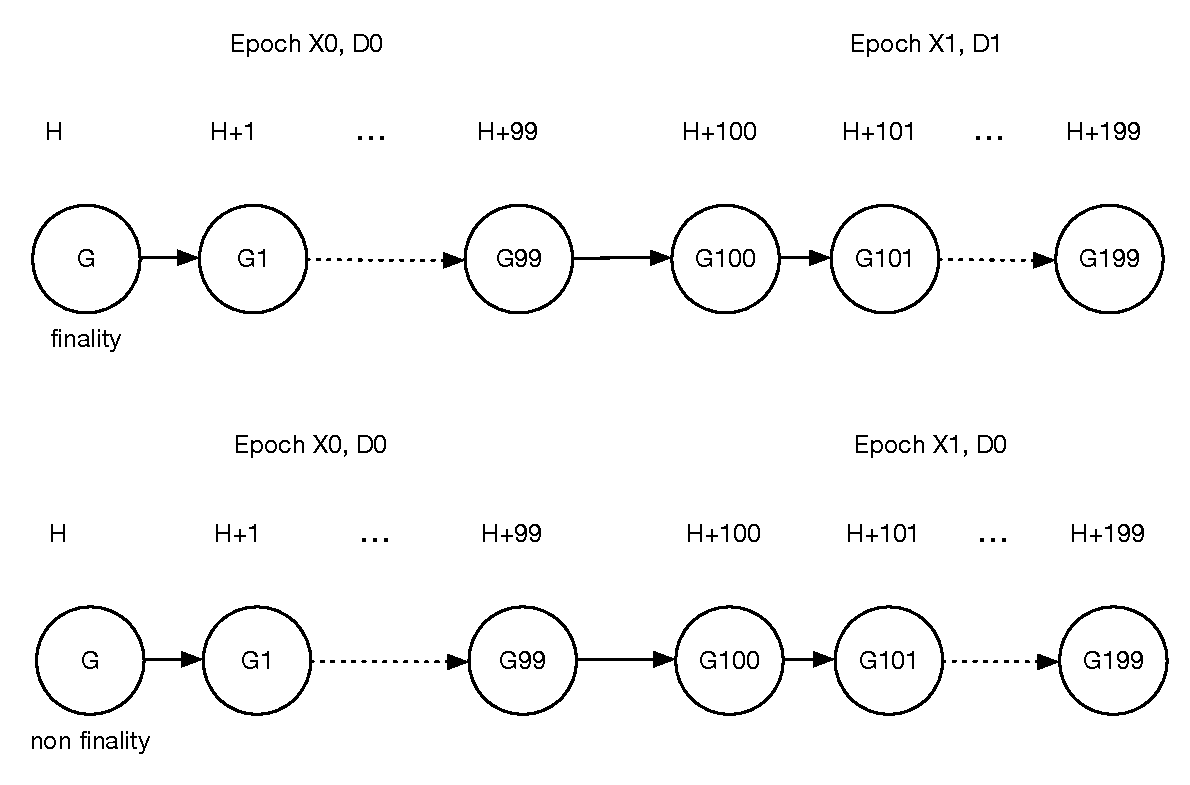
\includegraphics[width=8cm]{./figs/epoch}
\caption{验证者朝代更迭(假设X=100)}
\label{fig:epoch}
\end{figure}

由于网络延迟,各个节点可能在朝代更迭时,看到的区块G是否finality的状态不一致,所以参考Casper的动态验证集策略,要求每一个朝代的共识过程将由当前朝代和上一个朝代的验证者集合共同完成。因此在任意一个朝代,有资格的账户只能申请加入或者退出D+2朝代的验证者集合,当朝代变更到D+2时,才可加入新区块的共识过程。

\subsubsection{共识过程}
\label{pod:design:consensus}

新的区块被提出后,当前朝代验证者集合中所有人将会参与一轮BFT (Byzantine Fault Tolerant)方式的投票,来确定此区块的合法性。在投票最开始,每一个参与此区块共识的验证者将会被从押金中收取$2x$ ($x$为激励奖金比例)的保证金,然后进入两阶段的投票过程。

\begin{itemize}
\item \textbf{第一阶段},所有验证者需要对新区块投$Prepare$票,投完$Prepare$票的验证者将获得$1.5x$的奖励,如果在当前朝代和上一个朝代中都有超过$2/3$的押金总额的验证者对新区块投了$Prepare$票,那么该区块进入投票的第二阶段。此处需要说明,新区块的提议者将被默认对新区块投$Prepare$票。

\item \textbf{第二阶段},所有验证者需要对新区块投$Commit$票,投完$Commit$票的验证者,可以再获得$1.5x$的奖励,如果在当前朝代和上一个朝代中都有超过$2/3$的押金总额的验证者对新区块投了$Commit$票,那么该区块到达finality状态。
\end{itemize}

为了加速整个生态向前延展,如果区块b的$Prepare$和$Commit$票的时间戳和区块b的时间戳相差超过T,那么这些票将被视为过期,直接忽略。

\subsubsection{分叉选择}
\label{pod:design:fork}

PoD算法以每个高度上区块的得分来选择权威链,总是选择得分最高的区块加入权威链,在高度h的区块b的得分如下,

\begin{align}
Score(b, h) = \sum_{(b',h') \in children(b)}Score(b', h') + \sum committed~deposit~in~b
\end{align}
\noindent 即为该区块及其所有后代区块收到的commit票对应的押金总和,如图\ref{fig:fork_choice}所示。

\begin{figure}[h]
\centering
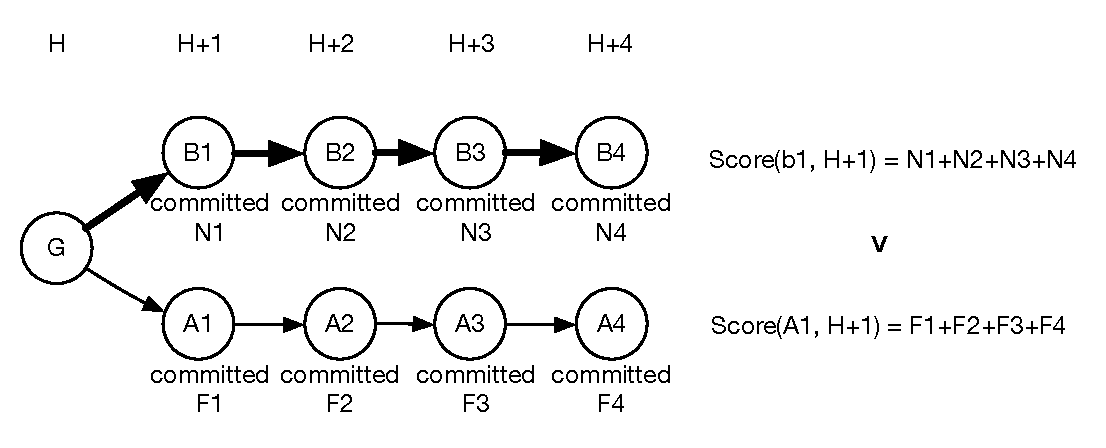
\includegraphics[width=12cm]{./figs/fork}
\caption{分叉选择}
\label{fig:fork_choice}
\end{figure}

\subsubsection{投票规则}
\label{pod:design:vote}

为了避免共识过程被恶意破坏,导致共识过程没法完成,阻碍生态发展,PoD参考Casper的最小惩罚规则~\cite{minimal_slash_rules}来约束验证者的共识活动。

假设共识过程中的$Prepare$和$Commit$票结构如下,
\begin{itemize}
\item $Prepare(H, v, vs)$,其中$H$为当前区块hash,$v$表示当前区块高度,$vs$表示$v$的某个祖先区块高度
\item $Commit(H, v)$,其中H为当前区块hash,$v$表示当前区块高度
\end{itemize}

PoD算法为整个投票过程制定了如下4条基本规则,

\begin{itemize}
\item 单个区块的两阶段共识过程存在严格的先后顺序,只有在第一阶段$Prepare(H, v, vs)$票总权值达到$2/3$后,验证者们才可以投出第二阶段的$Commit(H, v)$票,
\item 多区块间不强制一个区块共识结束后才能开始后一个区块的共识,允许交织共识(interwoven consensus),但是不能完全没有秩序,只有高度vs完成了第一阶段过程,拥有$2/3$的$Prepare(H_anc, vs, vs’)$后,才可以基于vs对其后代区块投$Prepare(H, v, vs)$票,保证交织稳步向前
\item 为了避免有节点利用交织共识恶意跨多区块投票,要求基于高度u投出了$Prepare(H, w, u)$票之后,对于高度在跨度u和w之间的所有区块,不能再投出$Commit(H, v)$票,保证共识过程的高效有序
\item 为了制止节点用同一笔押金在多个分支上同时下注,导致nothing~at~stake的问题,要求在一个高度投出$Prepare(H1, v, vs1)$票之后,不能再投出不一样的$Prepare(H2, v, vs2)$票
\end{itemize}

违反上述规则的验证者一旦被举报核实,将会被罚掉所有押金,举报者们将会共享罚金的4\%作为奖励,罚金的剩余部分将会被销毁。

\subsection{PoD经济分析}
\label{pod:economic}

\subsubsection{激励分析}
\label{pod:economic:incentive}

参与PoD算法的验证者,在每一个合法区块上可以获得1x的星云币奖励,如果网络不畅或者有人作弊导致Prepare阶段没有办法完成进入Commit阶段,那么所有验证者将损失0.5x。因此成为验证者的价值节点在保持网络畅通,不参与作弊的情况下,将共享大量记账收益。

\subsubsection{作弊分析}
\label{pod:economic:fraud}

\subsubsection*{双重支付攻击(double spend)}
\label{pod:economic:fraud:double_spend}

假设商户merchant等到新区块到达finality状态就确认交易发货,那么fraud要在PoD共识算法下完成双重支付攻击实现零成本购物要付出的最小代价如下:

首先,fraud需要提高自己的Nebulas Rank到Top N,然后缴一定数的NaS作为押金成为验证者,并申请参与D+2朝代区块的验证。

然后,fraud需要被伪随机算法选中为新区块的提议者,此时fraud提出两个高度相同的新区块,一个哈希值为hash1包含fraud向merchant的转账交易,另一个哈希值为hash2包含fraud向fraud自己的转账交易。

最后,为了让hash1和hash2区块都到达finality,如图\ref{fig:double_spend}所示,fraud至少需要花费所有押金的$1/3$来贿赂$1/3$的验证者,让他们给两个区块都投$Commit$票。

\begin{figure}[h]
\centering
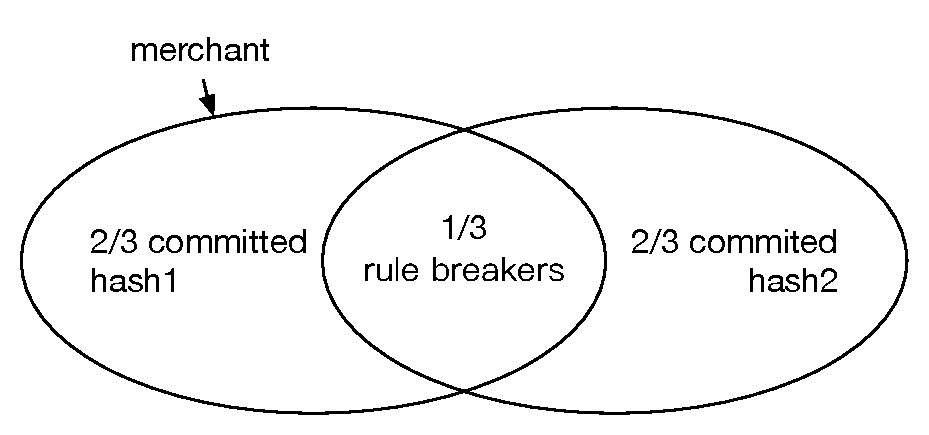
\includegraphics[width=7cm]{./figs/overlap}
\caption{双重支付经济惩罚}
\label{fig:double_spend}
\end{figure}

所以要完成一次成功的双重支付攻击,fraud需要花费一定的精力和财力来提升自己的Nebulas Rank排名(见\refsec{subsec:robust}抵抗操纵),然后等到幸运地被选为提议者时,至少花费总押金的$1/3$来让两个块同时到达finality状态。

\subsubsection*{51\%攻击(51\% attack)}
\label{pod:economic:fraud:51attack}

在PoW中要发起51\%攻击需要51\%的算力,在PoS中则需要51\%的押金,而在PoD中,则需要验证者集合中51\%的账户,这意味着拥有足够多的高声望用户进入Nebulas Rank的Top N,并且需要支付对应的押金,因此在PoD中51\%攻击将更为困难。

\subsubsection*{短程攻击(short-range attack)}
\label{pod:economic:fraud:short_range_attack}

PoD中的每个高度上的区块都有共识有效期,如果某个高度距离最新高度超过100时,该高度的所有区块在共识过程中将被视为过期,那么这些区块上的所有新的共识活动将会被直接忽略。因此要在PoD中完成长程攻击(long-range attack)几乎不可能,但是在有效期内依旧存在发起短程攻击的可能性。

短程攻击者Attacker试图在高度H+1的区块还没有过期的情况下,伪造A链来替代B链成为权威链,Attacker需要让区块A1的得分比B1更高。由于多投会被严惩,所以Attacker将不可避免地要贿赂验证者,否则无法完成短程攻击。为了展现PoD共识算法的安全性,下面分别分析使不同数量的区块失效时,Attacker需要付出的代价。

如果Attacker想要使B1失效,最小代价的情况如图\ref{fig:revert1},就相当一次双重支付攻击,Attacker幸运地成为了H+1高度的区块提议者,那么至少需要贿赂朝代D0中$1/3$的验证者多投使A1达到finality,最小代价为所有押金的$1/3$。

\begin{figure}[h]
\centering
\includegraphics[width=11cm]{./figs/revert1}
\caption{短程攻击使一个区块失效的情形}
\label{fig:revert1}
\end{figure}

如果Attacker想要使B1-B2失效,假设B1和B2都已到达finality,块中交易都已生效,为了让这些交易失效,这里考虑两种情况。第一种如图\ref{fig:revert2}中(a)所示,高度H+1和H+2在同一个Epoch中,朝代相同,那么Attacker首先需要贿赂D0中$1/3$的验证者使A1达到finality,此时这$1/3$的验证者将会被惩罚,押金被罚完。在A2的验证中整体押金总和只有A1中的$2/3$,此时Attacker想要让A2到达和B2同价值的committ票,需要贿赂剩下所有没有作弊的验证者,合起来至少需要损失总押金的$3/3$,即使如此也不能保证A1得分比B1高,攻击失败风险高。第二种情况如图\ref{fig:revert2}中(b)所示,高度H+1和H+2正好在不同的Epoch中,且朝代不相同,那么此时Attacker需要贿赂D0中的$1/3$来让A1到达finality,然后贿赂D1中的$1/3$来让A2达到finality,完成一次这样的攻击至少需要损失总押金的$2/3$。综上,想要发起短程攻击导致两个finality区块失效,至少需要花费总押金$2/3$的代价。

\begin{figure}[h]
\centering
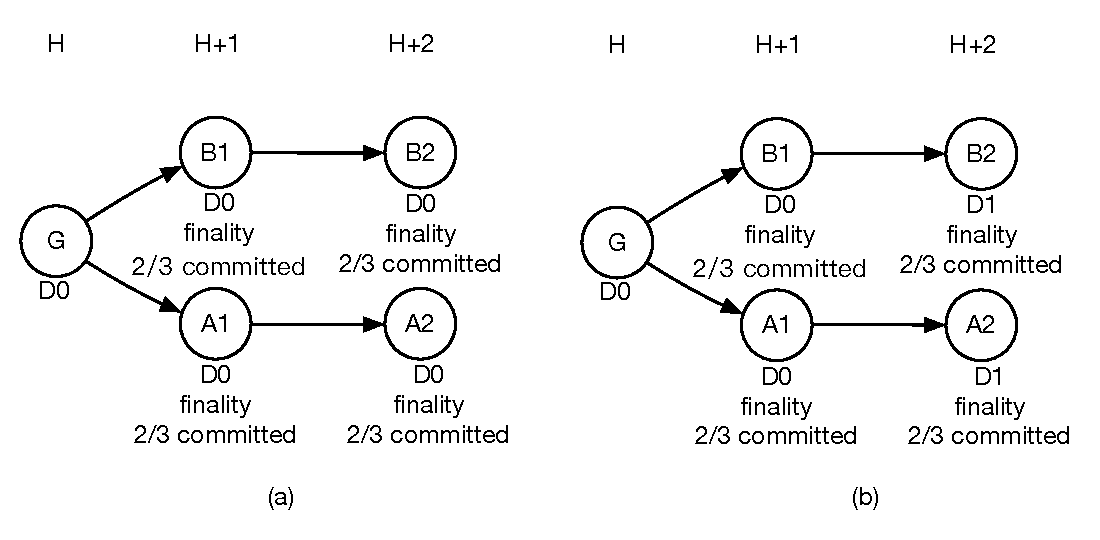
\includegraphics[width=11cm]{./figs/revert2}
\caption{短程攻击使两个区块失效的情形}
\label{fig:revert2}
\end{figure}


如果Attacker想要使B1-B3失效,如图\ref{fig:revert3}所示,Attacker首先需要贿赂D0中$1/3$的人完成A1的finality,然后贿赂D1中$1/3$的人完成A2的finality,最后需要贿赂D1中剩下$2/3$中的所有人来完成A3的finality,综上至少要损失总押金的$4/3$。要完成这些攻击准备将会十分困难,而且即使有幸做到了,也不定能保证A1的得分比B1高,攻击也可能会失败。

\begin{figure}[h]
\centering
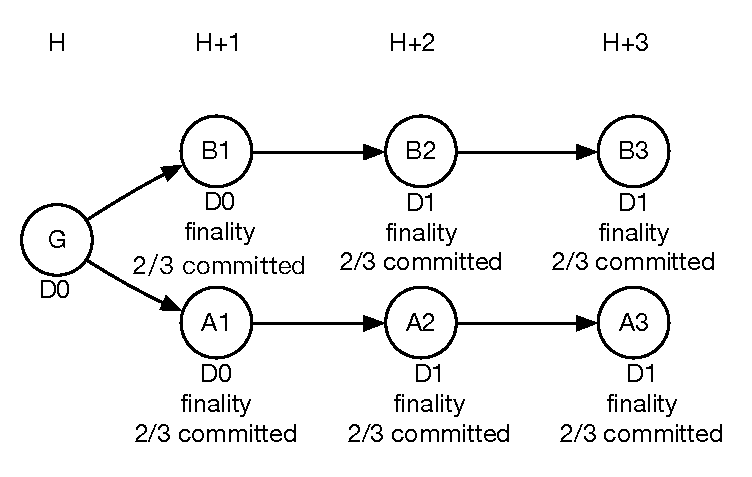
\includegraphics[width=7.5cm]{./figs/revert3}
\caption{短程攻击使三个区块失效的情形}
\label{fig:revert3}
\end{figure}

如果Attacker想要使B1-BN失效,其中N受到区块共识有效期的限制,不会很大,由于$N=3$时当前朝代所有验证者的押金就会被全部罚完,所以$N>=4$时,将没法完成攻击让B1得分比A1高,使B1-BN失效,发起这样的攻击没有任何意义。

\newpage
\section{总结}
\label{sec:conclusion}

\subsubsection*{我们认为}

区块链从一种高度抽象的角度来看是一种\textbf{用去中心化的方式对于数据的确权},代币本身是对于\textbf{确权价值的载体}。互联网解决了数据的通讯问题,而区块链则在互联网上层进一步解决了数据的确权问题。区块链前所未有第一次让大家的数据真正变成自己的数据,而不再被BAT等大公司任意分析并使用。

以公有链为代表的区块链本质精神是:\textbf{社群+代币+工具}。社群本质上是自下而上,秉承的是开放、开源、共享、非盈利的理念,和现有自上而下的商业生态有着根本的不同。代币即是对于确权价值的载体,未来会有更多的应用场景,而远非是仅仅面向虚拟货币,电子现金的属性。工具仅仅是对于区块链应用场景具体技术实施,如缺少前两者的结合,其单独来看\textbf{并不能完全体现区块链系统的魅力所在}。

以公有链为代表的区块链体系才是区块链的未来,因为其本身所具有的“\textbf{非信任}”、“\textbf{无特权}”的基本特性才是区块链系统真正的价值所在。恰恰相反,作为联盟链/企业链大多具有“\textbf{基于信任}”和“\textbf{基于特权}”的属性,不能突破既有的范式,属于改良式创新。而公有链系统颠覆了既有的协作关系,属于\textbf{颠覆式创新},是区块链价值最大化的真正体现。

\subsubsection*{我们致力于}

作为全球首个区块链搜索引擎,星云链致力于\textbf{发掘区块链世界价值新维度},打造基于价值尺度的区块链操作系统、搜索引擎及其他相关扩展应用。

基于此,我们提出Nebulas Rank星云指数来构建区块链世界的价值尺度,设计Nebulas Force星云原力来赋予区块链自我进化的能力,推出Developer Incentive Protocol开发者激励计划和Proof of Devotion贡献度共识证明来激励区块链的价值升级,打造Nebulas Search Engine区块链搜索引擎来帮助用户发现区块链上沉淀的多维度价值。

\subsubsection*{我们坚信}

正在发生科技浪潮会带领人们抵达更为\textbf{自由、平等、和美好}的生活。区块链作为其中重要的技术之一,会愈来愈散发出其特有的光彩和能量。能参与并投身其中,是我们最大的快乐和成就。

类似互联网对于世界的改变,区块链也即将面对其用户/应用临界值爆发的阶段。区块链技术会是下一代“智能网络”的\textbf{基础协议},整体用户规模会在5-10年内达到或超过10亿。未来的5年内会面临重大的机遇与挑战!

在未来的巨大生态面前,在当下,不要问区块链能为你做什么,而是要问你能为区块链做什么。因为,\textbf{区块链本身就是生命体,区块链本身就是经济体}!在区块链技术探索的道路上,与诸君共勉!

\printbibliography

%\bibliography{reference}
\end{document}
